\setAuthor{Jaan Kalda}
\setRound{lahtine}
\setYear{2019}
\setNumber{G 7}
\setDifficulty{7}
\setTopic{TODO}

\prob{Niit relssidel}
\begin{wrapfigure}[7]{r}{0.3\textwidth}
	\vspace{-13pt}
	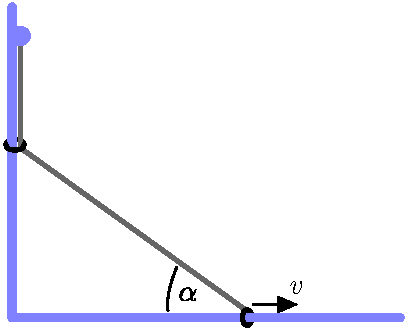
\includegraphics[width=0.3\textwidth]{2019-lahg-07-yl.pdf}
\end{wrapfigure}

Niit kogupikkusega $L$ on kinnitatud kahest üksteisega ristuvast lõigust koosneva relsi külge nii, nagu näidatud joonisel: üks ots on fikseeritud jäigalt vertikaalse relsiosa külge kaugusele $h$ relsi nurgast, alumine ots tillukese rõnga abil horisontaalse relsi külge. Niit on tõmmatud läbi teise tillukese rõnga, mis saab libiseda mööda vertikaalset relssi. Alumist rõngast liigutatakse konstantse kiirusega $v$. Leida teise rõnga kiirus ja kiirendus hetkel, mil nöör moodustab nurga $\alpha$ horisontaalsihiga.


\hint

\solu
Olgu alumise rõnga kaugus nurgast $x$ ja vertikaalse rõnga kaugus $y$, niidi pikkus $L$ ja kinnituspunkti kõrgus $h$. Sellisel juhul $x^2+y^2=(L+y-h)^2$, võttes siit ajalise tuletise saame $2x\dot x+2y\dot y=2(L+y-h)\dot y$, kus punkt sümboli kohal tähistab ajalist tuletist, st $\dot x=v$. Lihtsustades seda avaldist leiame $vx=(L-h)\dot y$. Esiteks saame siit avaldada otsitava kiiruse
$$
\dot y=vx/(L-h)=v\left(\frac{L+y-h}{x-\frac yx}\right)^{-1}=
$$
$$
=v/(\frac 1{\cos\alpha}-\tan\alpha)^{-1}=\frac{v\cos\alpha}{1-\sin\alpha}.
$$
Teiseks, kui võtame antud avaldisest veelkord tuletise, saame $v\dot x=(L-h)\ddot y$, millest kiirendus $\ddot y=v^2/(L-h)$. Pangem tähele, et kiirendus püsib konstantne.
\probend